\chapter{Computation of a capacitance matrix}


\modinfo{Directory}{CapacitanceMatrix}
\modinfo{Solvers}{\Idx{StatElecSolve}}
\modinfo{Tools}{\Idx{ElmerGrid}, Editor}
\modinfo{Dimensions}{2D, Steady-state}

\subsection*{Case definition}

\begin{flushleft}

In Elmer, a \Idx{capacitance matrix} is possible to solve with an algorithm where a unity potential is permutated through 
all bodies and the resulting charges are registered. 

In this case the capacitancies is solved between four different bodies (Figure \ref{fg:4holegeometry}). We have assumed that the model is manufactured from glass of dimensions 5 m height and length. Due to symmetry of the model each body has the height and length of 1 m. To solve the problem we only need to know the relative permittivity of glass (Table \ref{tb:glasspar}).

\begin{figure}[h]
\centering
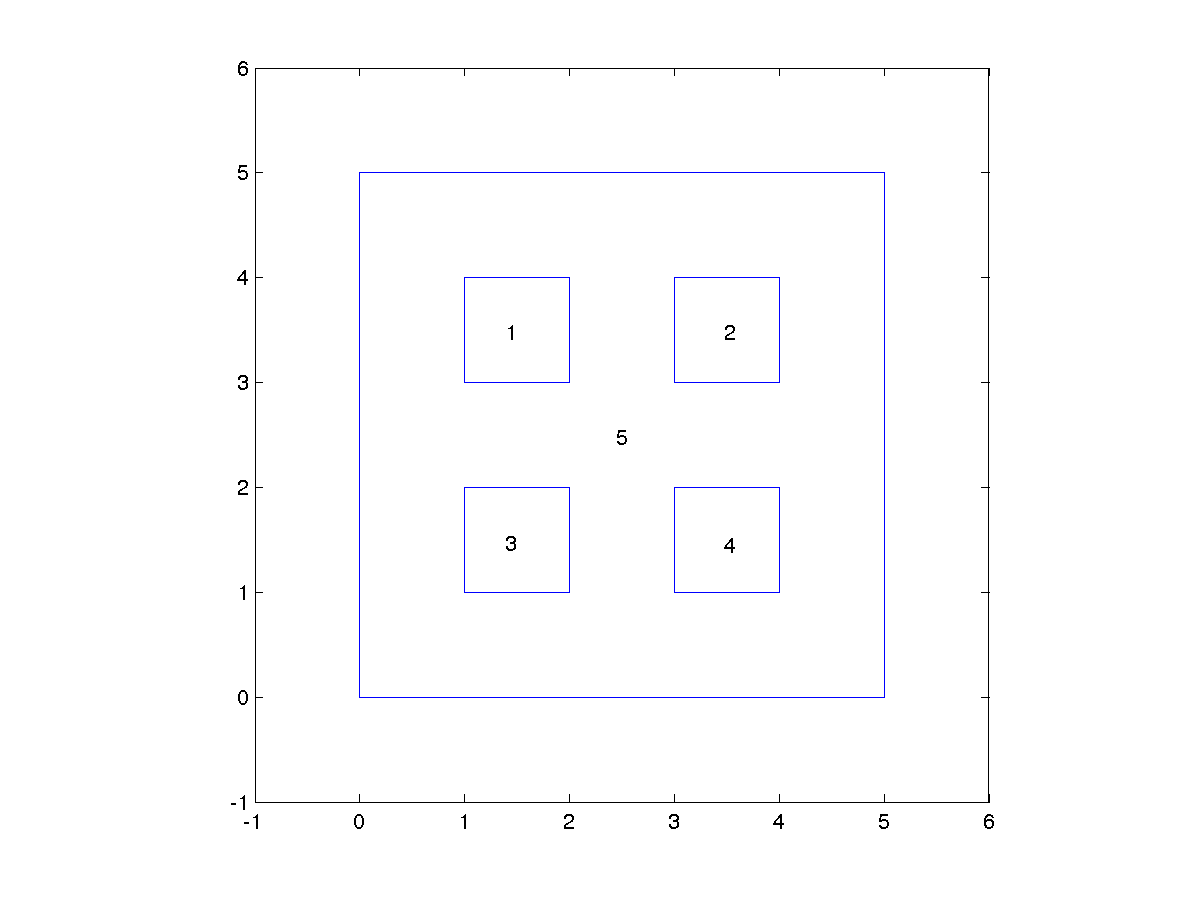
\includegraphics[height=80mm]{4holegeometry}
\caption{Geometry of the model.}\label{fg:4holegeometry}
\end{figure}


\begin{table}[h]
\caption{Material parameters.}
\label{tb:glasspar}
\begin{center}
\begin{tabular}{ll} \hline
parameter  & value \\ \hline
relative permittivity & 7      \\ \hline
\end{tabular}
\end{center}
\end{table} 


\end{flushleft}

\subsection*{Solution procedure}

\begin{flushleft}
Let us next introduce the solution procedure of the problem.
The computation mesh has been created with Gambit software and it consists of 15941 elements. The mesh can be convert into Elmer format with the command

\ttbegin
ElmerGrid 7 2 mesh.FDNEUT
\ttend

This command creates the directory {\tt mesh} which contains the mesh files. 

\ttbegin
Header
  Mesh DB "." "mesh"
End
\ttend

The simulation of the problem is carried out in a 2D cartesian geometry.
The different permutation are computed within the nonlinear iterations of the solver and therefore only one
steady state iteration is needed.

\ttbegin
Simulation
  Coordinate System = "Cartesian 2D"
  Simulation Type = "Steady"
  Output Intervals(1) = 1 
  Steady State Max Iterations = 1
  Output File = File "4_holes.result"
  Post File =   File "4_holes.ep"
End
\ttend

In the solver section the keyword {\tt Calculate Capacitance Matrix} must be set to {\tt True}. 
We also have to define the number of the bodies in our system. 
The calculated matrix is saved to file cmatrix.dat.

\ttbegin
Solver 1
  Equation = "Stat Elec Solver"
  Procedure = "StatElecSolve" "StatElecSolver"
  Variable = "Potential"
  Variable DOFs = 1
  Calculate Capacitance Matrix = Logical True
  Capacitance Bodies = 4
  Minimum CoEnergy = 1e-10
  Capacitance Matrix Filename = "cmatrix.dat"
  Linear System Convergence Tolerance = 1.0E-8
  Linear System Solver = "Iterative"
  Linear System Iterative Method = "BiCGStab"
  Linear System Max Iterations = 1000
  Linear System Abort Not Converged = True
  Linear System Preconditioning = ILU2
  Linear System Residual Output = 1
  Nonlinear System Convergence Tolerance =  1.0E-06
  Nonlinear System Max Iterations = 1
  Nonlinear System Relaxation Factor = 1.0
  Steady State Convergence Tolerance =  1.0E-04
End
\ttend

The body section is defined as follows

\ttbegin
Body 1
  Equation = 1
  Material = 1
End
\ttend                                      

If we want to write the electric energy density in the result file, the keyword {\tt Calculate Electric Energy} have to set to {\tt True}.      

\ttbegin                                                           
Equation 1
  Active Solvers =  1
  Calculate Electric Energy = Logical True
End
\ttend

We only need one material parameter of glass in our simulation.

\ttbegin               
Material 1
  Relative Permittivity = 7
End
\ttend

The final task is to specify the needed boundary conditions.
The keyword {\tt Capacitance Body} indicates whether the capacitance will be calculated or not.
The bodies, in which the capacitance is going to be computed, should number from 1 up to the value of the
{\tt Capacitance Bodies} in the solver section.
The ground may be given with value 0 for this keyword (or by setting the potential to zero).  

\ttbegin
Boundary Condition 1
  Target Boundaries = 1
  Capacitance Body = 1
End

Boundary Condition 2
  Target Boundaries = 2
  Capacitance Body = 2
End

Boundary Condition 3
  Target Boundaries = 3
  Capacitance Body = 3
End

Boundary Condition 4
  Target Boundaries = 4
  Capacitance Body = 4
End

Boundary Condition 5
  Target Boundaries = 5
  Capacitance Body = 0
End
\ttend

\end{flushleft}


\subsection*{Results}

\begin{flushleft}

Elmer writes the capacitance matrix to file cmatrix.dat.
Note that if the capacitance has been calculated between two different bodies, the calculated value appears two times in the matrix.
Elmer also outputs the calculated capacitancies on the screen, where they can be examined:

\begin{center}
\ttbegin
StatElecSolve: Capacitance matrix computation performed (i,j,C_ij)
StatElecSolve:   1  1    2.11054E-10
StatElecSolve:   2  2    2.11027E-10
StatElecSolve:   3  3    2.11015E-10
StatElecSolve:   4  4    2.11052E-10
StatElecSolve:   1  2    7.74093E-11
StatElecSolve:   1  3    7.74260E-11
StatElecSolve:   1  4    1.32739E-11
StatElecSolve:   2  3    1.32801E-11
StatElecSolve:   2  4    7.74067E-11
StatElecSolve:   3  4    7.74120E-11
StatElecSolve: Capacitance matrix was saved to file cmatrix.dat
\ttend 

$Capacitancies$ $(F)$.
\end{center}


\end{flushleft}




























